% Metódy inžinierskej práce

\documentclass[10pt,twoside,slovak,a4paper]{article}

\usepackage[slovak]{babel}
%\usepackage[T1]{fontenc}
\usepackage[IL2]{fontenc} % lepšia sadzba písmena Ľ než v T1
\usepackage[utf8]{inputenc}
\usepackage{graphicx}
\usepackage{url} % príkaz \url na formátovanie URL
\usepackage{hyperref} % odkazy v texte budú aktívne (pri niektorých triedach dokumentov spôsobuje posun textu)

\usepackage{cite}
%\usepackage{times}

\pagestyle{headings}

\title{Jedinečné svetlené efekty v hrách\thanks{Semestrálny projekt v predmete Metódy inžinierskej práce, ak. rok 2022/23, vedenie: Igor Stupavský}} % meno a priezvisko vyučujúceho na cvičeniach

\author{Branislav Fech\\[2pt]
	{\small Slovenská technická univerzita v Bratislave}\\
	{\small Fakulta informatiky a informačných technológií}\\
	{\small \texttt{xfech@stuba.sk}}
	}

\date{\small 28. september 2022} % upravte



\begin{document}

\maketitle

\begin{abstract}
Prvotriedne spracovanie istých svetelných efektov je kritické v modernom hraní. 
Jeho nedôveryhodnosť je schopné nevedome zruinovať zážitok z hry. Väčšina z nás 
si to ani nemusí uvedomiť, môžeme mať len pocit, že niečo nesedí a často krát 
nehodnovernosť svetelného spracovania ničí pocit realizmu danej hry. Avšak ani 
moderná technológia prístupná obyčajnému človeku nie je schopná spracovať každú 
časticu zvlášť, teda aspoň nie v zlomku sekundy. Preto je potrebné spracovať tieto 
efekty čo najdôveryhodnejšie, avšak zároveň s čo najmenšou záťažou na naše hardware-ové 
vybavenie.
\ldots
\end{abstract}



\section{Úvod}
Málokto by nesúhlasil s tvrdením, že svetlo je jednou z, ak nie najdôležitejšou 
zložkou skvelo graficky spracovanej hry. Narozdiel od nedokončených textúr, alebo 
nedostatku detailov, svetlo možno nespozorujeme na prvý pohľad. Môžeme si len povedať, 
že je niečo inak, ako by malo byť a už to robí hrou menej hodnotnou. V tejto práci sa 
budem zameriavať na zložitejšie prípady svetelných efektov a spôsoby ich vyobrazenia.

\section{Svetelné efekty} \label{se}
Svetlo sa neustále odráža alebo láme od všetkých hmotných vecí. Väčšina svetelných 
efektov pre nás nie je ničím zaujímavá, keďže sa s nimi stretávame každý deň. Sú ale 
aj také, pri ktorých si môžeme povedať, že sme sa ocitli v správny čas na správnom mieste.
Tieto efekty dodávajú  pozorvateľovi uchvacujúci a jedinečný pocit, teda robia daný 
moment viac pamätania hodný.

\subsection{Kaustika} \label{se:kaustika}
Kaustika je jedným zo svetelných efektov, ktoré môžeme pozorovať napríklad keď svetlo 
prechádza pohárom, alebo na dne bazéna za predpokladu, že voda je číra. Vzniká, keď sa 
svetlo odráža alebo sa láme pri prechode médiom a tieto lúče sa zbiehajú v jednom mieste, 
teda daná plocha je viac osvetlená.

\subsection{Svetelné lúče} \label{se:luce}
Svetelné lúče je možné pozorovať v scenérii, kedy je väčšina svetla blokovaná istým 
objektom, napríklad stenou. Avšak časť svetla, ktorá nie je blokovaná, napríklad svetlo 
prechádzajúce oknom, alebo deravou strechou, je viditeľná v podobne jedného alebo viacerých 
svetelných lúčov. To vytvára kontrast medzi tmavou časťou scenérie a jedným alebo viacerými 
svetelnými lúčmi.

\subsubsection{Krepuskulárne lúče} \label{se:luce:kl}
Krepuskulárne lúče sú špecifickým prípadom výskytu svetelných lúčov. V tomto prípade 
svetlo nie je blokované pevným objektom, ale oblakmi. Čo robí tento prípad svetelných 
lúčov zaujímavým a pre výpočtovú grafiku náročným je skutočnosť, že oblaky nie sú 
nepriehľadné, ale priesvitné. Teda svetlo je pohlcované v iných množstvách, niekde 
viac a niekde menej, takže svetelné lúče sa vyskytujú v rôznych intenzitách. Narozdiel 
od svetla blokovaného budovou, kde sa môžu vyskytnúť len 2 prípady- buď svetlo prechádza, 
alebo nie.

\begin{figure}[h]
    \centering
    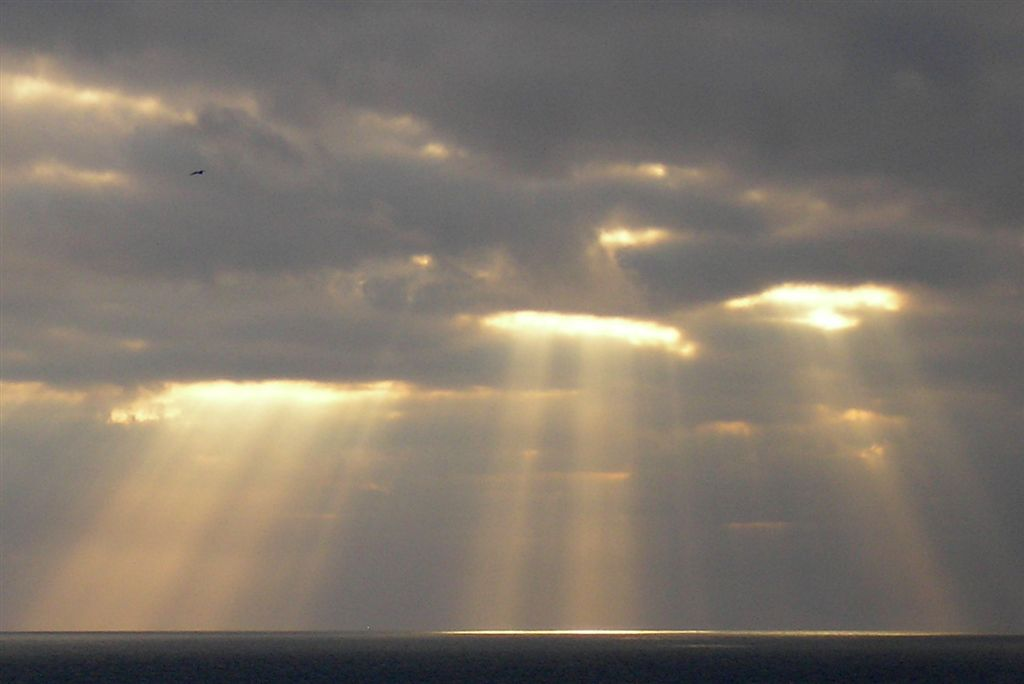
\includegraphics[scale=0.2]{god_ray.jpg}
    \caption{Krepuskulárne lúče}
    \label{fig:kl}
\end{figure}

\section{Spracovanie} \label{spracovanie}
V prípade spracovania krepuskulárnych lúčov na obyčajnej fotografii nie je zložitosť 
nejako vysoká, nakoľko výsledok nemusí byť hotový v zlomku sekundy. Avšak hry sú niečo 
iné. Úlohou je vypracovať daný obraz čo najhodnovernejšie a zároveň s čo najväčším 
realizmom.

\subsection{Post-processing} \label{spracovanie:pp}
Táto metóda je bohužiaľ funkčná len v prípade, že zdroj svetla sa nachádza v obraze, 
teda zlyhá, ak zdroj nie je viditeľný. Na druhej strane, výhoda tejto metódy spočíva v 
tom, že úprava obrázka nijako neovplyvňuje čas vykresľovania obrázka, nakoľko sú 
krepuskulárne lúče jednoduchými "efektami" len pridané do obrázka.

\subsection{Mapovanie tieňov} \label{spracovanie:mt}
V roku 2009 bola prednesená ďalšia metóda na spracovanie krepuskulárnych lúčov v reálnom 
čase pomocou mapovania tieňov. Tie slúžia na detekciu oklúzie alebo "prekážky" vo svetelných 
lúčoch. Tento algoritmus je síce schopný fungovať len v homogénnom prostredí, ale na druhej 
strane je schopné pracovať aj s dynamickým zdrojom svetla a taktiež dynamickými predmetmi 
pôsobiacimi ako oklúzie. Nakoľko je tento algoritmus náročný na výpočet, je v ňom 
implementované preložené vzorkovanie na zníženie výpočtovej doby.

\section{Porovnanie} 
\label{por}
Obe metódy spomenuté vyššie majú svoje výhody  a nevýhody.

Post processing nám prináša rýchlejšie zobrazenie, keďže úprava sa deje až po tom, čo 
je obraz vykreslený. Nevýhodou však je, že výsledky nemusia byť vždy úplné dôveryhodné 
a na to, aby tento algoritmus fungoval, musí byť zdroj svetla v obraze. 

V prípade použitia mapovania tieňov je nevýhodou pomalšie zobrazenie kvôli nutnosti 
mapovania každého svetelného lúča zvlášť. Výhody prinášané týmto algoritmom sú oveľa 
prirodzenejšie výsledky spolu s tým, že je schopný pracovať s pohyblivým svetelným 
zdrojom aj keď sa nenachádza v zornom poli hráča, narodziel od post-processingu.

\section{Zhrnutie} 
\label{zhr}
Dilemou je rozhodnúť sa medzi pomalším, ale prirodzenejším, alebo rýchlejším, ale 
menej uspokojivým výsledkom. Je logické držať sa blízko fyzicky korektného zobrazenia 
týchto svetelných efektov pre čo najlepšie výsledky. No vykresľovanie týchto scenérií 
v reálnom čase je aj v dnešnej dobe v stave, kedy je veľa miesta pre ďalší rozvoj.


%\acknowledgement{Ak niekomu chcete poďakovať\ldots}


% týmto sa generuje zoznam literatúry z obsahu súboru literatura.bib podľa toho, na čo sa v článku odkazujete
\bibliography{literatura}
\bibliographystyle{plain} % prípadne alpha, abbrv alebo hociktorý iný
\end{document}
